\documentclass[letterpaper,12pt]{article}
\usepackage{indentfirst}
\usepackage{fullpage}

\usepackage[pdftex, bookmarks, bookmarksopen=true, colorlinks=false,
pdftitle={SpaceFortress 5: Subject Instructions}]{hyperref}
\usepackage{graphicx}

\newcommand{\HRule}{\rule{\linewidth}{0.5mm}}

\begin{document}

\begin{titlepage}
\begin{center}
\null
\vfill
\textsc{\Large Subject Instructions}\\[0.5cm]
\HRule \\[0.7cm]
{ \huge \bfseries Space Fortress 5}\\[0.4cm]
\HRule \\[1.5cm]
\begin{minipage}{0.4\textwidth}
\begin{center} \large
Marc \textsc{Destefano}\\
Ryan \textsc{Hope}
\end{center}
\end{minipage}
\vfill
{\large \today}
\end{center}
\end{titlepage}

\thispagestyle{empty}
\begin{center}
\null
\vfill
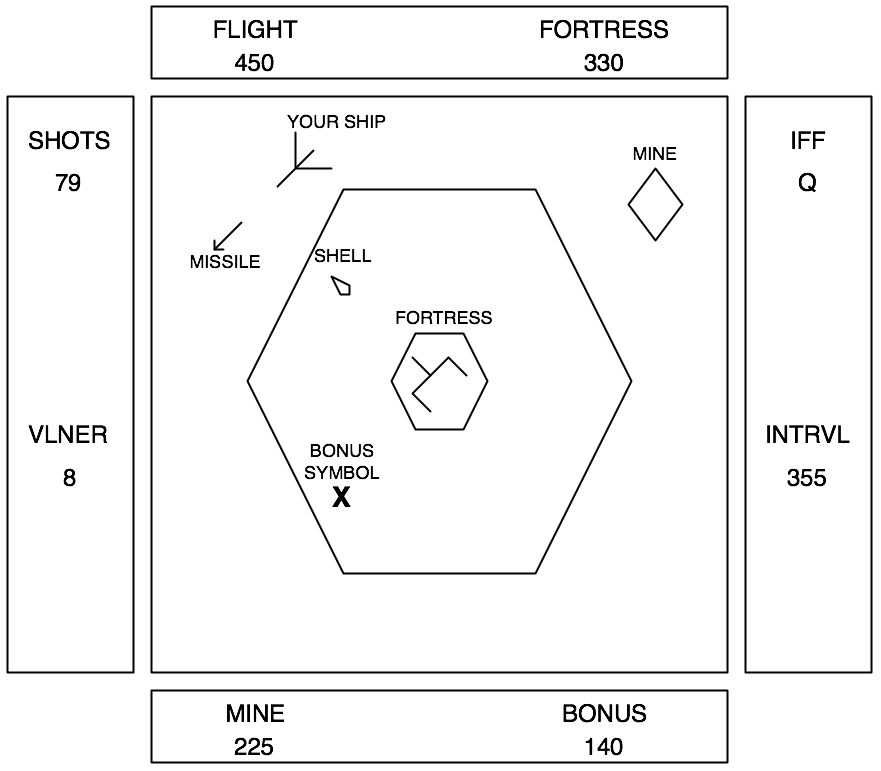
\includegraphics[width=\textwidth]{SF5.png}
\vfill
\end{center}
\newpage

\section{Introduction}

This game you will be playing is called ``\textbf{Space Fortress}''. It is a complex and difficult
game that requires a high degree of skill. You will be controlling a spaceship that is moving in a
frictionless environment which includes hostile elements: a fortress and mines which will try to
damage or destroy your spaceship. Your primary goal is to maximize your game points. To accomplish
this, you will have to:
\textbf{\begin{enumerate}
\item Destroy the Fortress as many times as you can
\item Hit as many mines as possible
\item Protect your own ship from being hit or damaged while moving slowly and carefully
\item Capture as many bonus opportunities as possible
\end{enumerate}}
On the computer display, the middle section represents the environment in which you will fly your
ship to accomplish your mission. An instrument panel is located surrounds the display which displays
information necessary for flight and mission performance.

\subsection{Your Spaceship}

Please point to the spaceship on the diagram now. You will be controlling the motion of your
spaceship with the keyboard. Remember that the ship is moving in a frictionless environment, and is,
thus, very sensitive to input. Pressing the ``W'' key will cause the ship to accelerate in the
direction in which it is pointing. Pressing the ``A'' or ``D'' keys will rotate the ship
counter-clockwise or clockwise, respectively. Pressing the ``S'' key will have no effect on the
movement of the ship. You should realize that the ship will not slow down or stop unless you
accelerate it in the direction opposite to that in which it is presently moving.

The boundaries of the region in which you should try to fly your ship are represented by
two hexagons displayed on the screen. Please point to the hexagons now.

Your ship will be moving in a hostile environment in which it is constantly threatened by the
fortress and mines. After your ship has been damaged four times, it will be destroyed and the game
will start again automatically. To defend yourself, your ship comes equipped with missiles which you
may fire at either the fortress or mines. The firing button is the space bar on your keyboard. When
you press the space bar it will fire a missile in the direction in which the ship is pointing. Your
ship can carry no more than 100 missiles.

\subsection{The Fortress}

In this game, your principal opponent is the fortress which is stationed in the center of the
screen. Please point to the fortress now. The fortress can rotate, track, and lock onto your ship,
firing a shell at your ship after a short delay. When a shell hits or passes very close to your
ship, it will damage or destroy your ship.

Your mission is to destroy the fortress. In order to do this, you have to hit the fortress with your
missiles at least 10 times. The number of fortress hits is displayed in the ``\textbf{Vulnerability
Counter}'' (\textbf{VLNER}) on the instrument panel. Please point to the \textbf{VLNER} counter now.
Once you hit the Fortress 10 times, it becomes vulnerable. Now you can destroy it by hitting it with
a double shot – that is, two consecutive shots within 250 milliseconds of each other. It is okay to
wait until you have hit the Fortress more than 10 times before you attempt the double shot. However,
if you have hit it fewer than 10 times, and you fire a double shot at it, the \textbf{VLNER} counter
will reset back to zero and you have to start accumulating Fortress hits all over again.

\subsection{Mines}

Mines constitute an additional threat to your ship. Approximately every 10 seconds, a mine will
appear somewhere on the screen. Please point to the mine now. A mine will actively pursue your ship
and try to damage or destroy it if it collides with your ship. You can destroy a mine by firing at
it. If you do not destroy the mine, it will remain active for 10 seconds before it disappears.

A mine can be either ``Type 1'' or ``Type 2''. Its type is identified by a letter that appears in
the middle of the instrument panel under the label \textbf{IFF} (Identify Friend or Foe). Please
point to the \textbf{IFF} indicator now. Before each 5-minute game, three letters will be displayed
on the screen that designate the identities of the ``Type 2'' mines. These identifiers will change
from one game to the next. It is very important that you remember these letters. When you detect a
mine on the display, check your instrument panel. If the letter is one of the three letters
presented at the beginning of the game, the mine on the display is ``Type 2''. If the letter is not
one of the three presented at the beginning, then it is ``Type 1''.

When you fire your missile at a Type 1 mine, you will ``energize'' it. Each time you energize a Type
1 mine you will receive 20 points to your Mine score and the vulnerability counter will increment by
one point; energizing Type 1 mines increases the vulnerability of the Space Fortress.

Your weapon system is ineffective against Type 2 mines until you have properly identified them. In
order to identify a mine as Type 2, you have to press the IFF button (the “J” key on the keyboard)
two times. The interval between the two key presses must be between 250 and 400 milliseconds. Any
interval that is shorter or longer than this range will not be effective. On the right side of the
instrument panel, a counter displays the actual interval between your two button presses
(\textbf{INTRVL}). Please point to the \textbf{INTRVL} counter now. If you did not succeed in
hitting the two key presses at the right interval, you can try again. Each time you destroy a Type 2
mine, you receive 30 points to your Mine score.

\textbf{To summarize:} A mine appears, you check the letter under IFF. If the mine is Type 1, aim
and press the space bar. If it is a Type 2, press the ``J'' key twice with the two presses within
250-400 msec, then aim and press the space bar.

\textbf{IMPORTANT!} When a mine appears on the screen, your weapon is not effective against
the fortress. However, once the mine disappears (or you have destroyed it), your weapons system
automatically becomes effective against the fortress again.

\textbf{Possible Errors in Mine Identification:}
\begin{enumerate}
\item The mine is Type 1 and you press the IFF button.
\begin{itemize}
\item Your weapon system becomes ineffective and all you can do is avoid the mine and them fortress
and wait until the mine disappears (10 seconds after its appearance).
\end{itemize}
\item The mine is Type 2 and you do not press the IFF button.
\begin{itemize}
\item Your weapon system remains ineffective, but you can still identify the mine with the IFF
button, after which your weapon system becomes effective and you can shoot the mine.
\end{itemize}
\item The mine is a Type 2, you press the IFF button twice, but the interval between button presses
was too long or too short.
\begin{itemize}
\item Your weapon system is ineffective, but you can try the double button press again.
\end{itemize}

\end{enumerate}

\subsection{Resource Limitations}

When the game begins, you have 100 missiles. The number of missiles your ship has
remaining is displayed in the ``\textbf{SHOTS}'' counter on the left side of the instrument panel.
Please point to the \textbf{SHOTS} counter now. Once your supply is depleted, you can still shoot,
but every missile that you shoot will cost you 3 points.

\subsection{Bonus Opportunities}

Surrounding the fortress, different symbols will appear (``\textbf{A}'', ``\textbf{B}'',
``\textbf{X}'', ``\textbf{Y}''). Please point to the symbol now. When an ``\textbf{A}'' is followed
by an ``\textbf{X}'', you have the opportunity to obtain more resources. You can choose to get 100
Bonus points, or up to 50 missiles plus 50 Bonus points. The choice is yours. You will have to
decide each time which choice will be of more benefit.
\begin{itemize}
\item Select 50 missiles and 50 Bonus points by pressing the ``K'' key.
\item Select 100 Bonus points by pressing the ``L'' key.
\end{itemize}
 
If you press one of these buttons after the ``\textbf{X}'' that follows an ``\textbf{A}'', and
before the next symbol appears, you will get the bonus that you selected and you will hear a chime.
However, if you press one of these two buttons at any other time, including after an ``\textbf{A}''
but before the next symbol appears, you will hear a buzzing sound and lose 50 Bonus points.
Furthermore, if you hit one of the buttons following an ``\textbf{A}'' and the next symbol happens
to be an ``\textbf{X}'', hitting one of the bonus keys will have no effect.

\subsection{Ship Control}

You must learn to acquire control of the ship and fly it in a planned trajectory. Your goal
is to fly the ship in a clockwise direction around the fortress while staying within the hexagon
boundaries. By doing this, you will maximize your Ship points.

\section{Scoring}

\subsection{Flight}

Your total number of points for this subscore is continuously updated and displayed on
the instrument panel underneath the label ``\textbf{FLIGHT}''. Please point to the \textbf{FLIGHT}
counter on the top of the instrument panel now.\\

\noindent
Points will be added to your \textbf{Flight} score as follows:
\begin{itemize}
\item 6 points/second – when your ship is on the screen, and within the hexagon
boundaries
\item 3 points/second – when the ship is on the screen, but outside the hexagon
boundaries
\item 7 points/second for moving at a low velocity
\end{itemize}

\noindent
Points will be subtracted from your \textbf{Flight} score as follows:
\begin{itemize}
\item -7 points/second for moving at a fast velocity
\item -35 points every time your ship leaves the screen and ``warps'' to the other side
\item -5 points every time your ship bounces off the inner hexagon
\end{itemize}

\subsection{Fortress}

Your total number of points for this subscore is continuously updated and displayed on
the instrument panel underneath the label ``\textbf{FORTRESS}''. Please point to the
\textbf{FORTRESS} counter on the top of the instrument panel now.\\

\noindent
Points will be added to your \textbf{Fortress} score as follows:
\begin{itemize}
\item 100 points when you destroy the Fortress
\end{itemize}

\noindent
Points will be subtracted from your \textbf{Fortress} score as follows:
\begin{itemize}
\item -50 points if a shell from the fortress damages your ship
\item -100 points if a shell from the fortress destroys your ship
\end{itemize}

\subsection{Mine}

Your total number of points for this subscore is continuously updated and displayed on
the instrument panel underneath the label ``\textbf{MINE}''. Please point to the \textbf{MINE}
counter on the instrument panel now.\\

\noindent
Points will be added to your \textbf{Mine} score as follows:
\begin{itemize}
\item 20 points for destroying a Type 1 mines
\item 30 points for destroying a tagged Type 2 mine
\end{itemize}

\noindent
Points will be subtracted from your \textbf{Mine} score as follows:
\begin{itemize}
\item -50 points if the mine ``times out'' (disappears before you destroy it)
\item -50 points if a mine damages your ship
\item -100 points if a mine destroys your ship
\end{itemize}

\subsection{Bonus}

Your total number of points for this subscore is continuously updated and displayed on
the instrument panel underneath the label ``\textbf{BONUS}''. Please point to the \textbf{BONUS}
counter on the instrument panel now.\\

\noindent
Points will be added to your Bonus score as follows:
\begin{itemize}
\item 100 points for hitting the “L” key when a bonus is available
\item 50 points (and 50 missiles) for hitting the “K” key when a bonus is available
\end{itemize}

\noindent
Points will be subtracted from your Bonus score as follows:
\begin{itemize}
\item -50 points for hitting the “K” or “L” key when a bonus is not available
\item -3 points for firing a missile when the SHOTS counter is 0
\end{itemize}\\

\noindent
\textbf{Remember}, your main goal is to obtain the highest Total Score. Your Total Score is a
combination of the following four subscores: Flight, Fortress, Mine, and Bonus. To maximize the
points in each of these categories, you must do the following:

\begin{itemize}
\item \textbf{Flight:} Move the ship at a low velocity (speed). Stay on the screen and move
clockwise within the hexagon boundaries
\item \textbf{Fortress:} Hit and destroy the fortress as many times as possible. Avoid letting your
ship get hit or destroyed by shells.
\item \textbf{Mine:} Destroy as many mines as possible. Avoid letting your ship get hit or destroyed
by mines.
\item \textbf{Bonus:} Select the bonus points whenever possible except when the SHOTS counter is
below 50.
\end{itemize}

\begin{center}
\textbf{You will not know your Total Score for a game until it has ended.}
\end{center}

\section{Optimal Strategies}
\begin{enumerate}
\item Navigation
\begin{itemize}
\item circle the Space Fortress slowly in a clockwise direction while staying within the region
enclosed by the two hexagons.
\end{itemize}
\item Mine Responses for Correctly Identified Mines
\begin{itemize}
\item let the mines come to the ship, then turn and fire when they are close.
\end{itemize}
\item Mine Response for Incorrectly Identified Mines
\begin{itemize}
\item a Type 1 mine becomes indestructible if the foe response is made when it appears, that
is, if the IFF button is pushed.
\item if this happens, it cannot be destroyed and it can destroy the ship
\item in this situation, it is best not to run from the mine, stay on your hexagon course and let
the mine destroy your ship.
\end{itemize}
\item Missile Management
\begin{itemize}
\item when bonus opportunities occur, take points unless this ship has fewer than 50 missiles
remaining.
\end{itemize}
\end{enumerate}


\clearpage
\section{Summary of Instructions}
\noindent
\textbf{Ship Control:}
\begin{itemize}
\item You cannot slow down or stop the ship by pressing the “S” key. Also, pressing the
“thrust” key along with a “turn” key will not cause the ship to move diagonally.
\item To slow or stop the ship, remember to rotate the ship so that it is facing opposite its
current direction and apply slight thrust.
\end{itemize}
\textbf{Fortress:}
\begin{itemize}
\item Vulnerability score must reach 10 before the fortress can be destroyed.
\item Vulnerability points are accumulated by shooting the fortress and Type 1 mines.
\item When the vulnerability counter reaches 10 or more, a rapid double shot will destroy the
fortress.
\item BUT, if you fire a rapid double shot before the VLNER counter reaches 10, the counter
will reset to 0.
\end{itemize}
\textbf{Mines:}
\begin{itemize}
\item Every time a mine appears on the screen, a letter will appear under the IFF label on the
instrument panel.
\item The 3 letters that represent foe mines are displayed on the screen before each game.
\item When the mine on the screen is a Type 2 mine, you must press the “J” key twice with
an interval between key presses of 250-400 milliseconds. This interval is displayed on
the instrument panel under the label INTRVL next to the IFF label. If you do not obtain
the correct interval, you may try again as many times as you can.
\item When the mine on the screen is a Type 1 mine, all you have to do is shoot it to energize
it. BUT, if you press the IFF key, you will not be able to destroy the mine.
\item Missiles are not effective against the fortress while mines are on the screen.
\end{itemize}
\textbf{Resources and Bonuses:}
\begin{itemize}
\item You begin each new game with 100 missiles.
\item During the game, various symbols will appear on the screen beneath the Fortress
\item Every time an “A” is followed by an “X” symbol, you can select a bonus of 100 points
by pressing the “L” key, or a bonus of 50 missiles and 50 points by pressing the “K”
key.
\item BUT, if the “K” or “L” keys are pressed anytime before an “X” appears after an “A”,
the bonus for that pair of symbols is forfeited and you must wait for the next pair to
appear.
\end{itemize}

\end{document}          
